\documentclass[tikz,border=4pt]{standalone}
\usetikzlibrary{positioning}
% Graph for Unit 4.3, Problem 4 (replaces WS9a_Graph1).
% Curve is a piecewise cubic (Hermite/Bezier) through:
%   B=(2,0.8) horizontal tangent, D=(4,0) horizontal tangent, F=(6,2.1) horizontal tangent,
%   crossing the x-axis at G=7. Concavity changes at B, C (x=3), and E (x=5).
\begin{document}
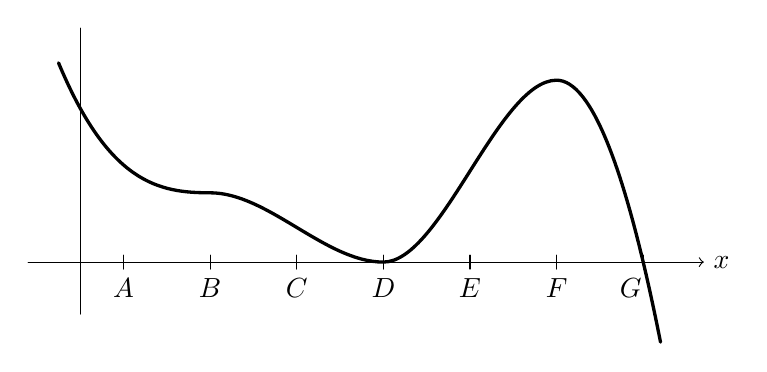
\begin{tikzpicture}[xscale=1.1,yscale=1.1,line cap=round]
  % axes
  \draw[->] (-0.1,0) -- (7.7,0) node[right] {$x$};
  \draw (0.5,-0.6) -- (0.5,2.7);
  % ticks and labels
  \foreach \x/\lab in {1/A,2/B,3/C,4/D,5/E,6/F} {
    \draw (\x,0.08) -- (\x,-0.08) node[below] {$\lab$};
  }
  \draw (7,0.08) -- (7,-0.08) node[below left=0pt and -3pt] {$G$};
  % the curve
  \draw[very thick]
    (0.25,2.3) .. controls (0.8333,0.9) and (1.4167,0.8) ..
    (2,0.8)    .. controls (2.6667,0.8) and (3.3333,0) ..
    (4,0)      .. controls (4.6667,0) and (5.3333,2.1) ..
    (6,2.1)    .. controls (6.4,2.1) and (6.8,1.092) ..
    (7.2,-0.924);
\end{tikzpicture}
\end{document}
